\documentclass[12pt]{article}
\usepackage{geometry}
\geometry{letterpaper, margin=1in}
\usepackage{titlesec}
\titleformat{\section}{\normalfont\Large\bfseries}{\thesection}{1em}{}
\titleformat{\subsection}{\normalfont\large\bfseries}{\thesubsection}{1em}{}
\usepackage{longtable}
\usepackage{graphicx}
\usepackage{tikz}
\usetikzlibrary{shapes,arrows,positioning}
\usepackage{hyperref}
\hypersetup{hidelinks}
\usepackage{array}
\usepackage{xcolor}

\title{Software Requirements Specification (SRS)\\
\large CanaLease Property Management Platform\\
\small D3 Submission}
\author{Chandanpreet Singh \\ Student ID: 40324569 \\ SOEN 6481 -- Systems Requirement Specification}
\date{August 1, 2025}

\begin{document}

\maketitle
\tableofcontents
\newpage

\section{Introduction}

This Software Requirements Specification (SRS) document provides a comprehensive description of the functional and non-functional requirements for the CanaLease Property Management Platform. This document follows the Unified Process (UP) methodology and includes a complete Use Case Model and Supplementary Specification.

\subsection{Purpose}
This SRS defines the complete system requirements for CanaLease, serving as the primary reference for developers, testers, project managers, and stakeholders throughout the development lifecycle.

\subsection{Scope}
The SRS covers all user interactions, system behaviors, performance requirements, and constraints for the CanaLease platform, a web-based property management system designed for the Canadian rental market.

\subsection{Document Organization}
\begin{itemize}
    \item Section 1: Introduction and overview
    \item Section 2: Use Case Model with detailed specifications
    \item Section 3: UML Diagrams (Use Case, Sequence, Activity, State Machine)
    \item Section 4: Supplementary Specification
    \item Appendices: Time logs, glossary, and supporting documentation
\end{itemize}

\section{Use Case Model}

\subsection{Actor-Goal List}

\begin{longtable}{|p{4cm}|p{10cm}|}
\hline
\textbf{Actor} & \textbf{Goal} \\
\hline
\endfirsthead
\hline
\textbf{Actor} & \textbf{Goal} \\
\hline
\endhead

Landlord/Property Manager & 
\begin{itemize}
    \item Add, edit, and remove properties from portfolio
    \item Manage rental units within properties
    \item Create and approve lease agreements
    \item Track rent payments and send reminders
    \item Assign and monitor maintenance tasks
    \item Communicate with tenants
    \item View financial reports
\end{itemize} \\
\hline

Tenant & 
\begin{itemize}
    \item Register and access tenant portal
    \item View lease information and documents
    \item Pay rent online securely
    \item Submit maintenance requests
    \item Track maintenance status
    \item Communicate with property manager
    \item View payment history
    \item Update personal information
\end{itemize} \\
\hline

Accounting Personnel & 
\begin{itemize}
    \item View rent collection summaries
    \item Record payments and adjustments
    \item Generate financial reports
    \item Export financial data
    \item Apply late fees and penalties
    \item Monitor outstanding balances
\end{itemize} \\
\hline

System Administrator & 
\begin{itemize}
    \item Manage user accounts
    \item Assign roles and access rights
    \item Configure system settings
    \item Monitor system performance
    \item Manage security settings
\end{itemize} \\
\hline

Maintenance Contractor & 
\begin{itemize}
    \item Receive work orders
    \item Update maintenance task status
    \item Submit completion reports
    \item Upload photos and documentation
\end{itemize} \\
\hline

Payment Gateway & 
\begin{itemize}
    \item Process payment transactions
    \item Validate payment information
    \item Provide transaction confirmations
\end{itemize} \\
\hline

Email System & 
\begin{itemize}
    \item Send automated notifications
    \item Deliver reminders and alerts
\end{itemize} \\
\hline
\end{longtable}

\subsection{Use Case Specifications}

% UC01: Add/Edit/Remove Property
\subsubsection{UC01: Add/Edit/Remove Property}

\begin{tabular}{|p{3cm}|p{11cm}|}
\hline
\textbf{Id:} & UC01 \\
\hline
\textbf{Use Case:} & Add/Edit/Remove Property \\
\hline
\textbf{Description:} & Landlord manages properties in their portfolio by adding new properties, editing existing property details, or removing properties from the system. \\
\hline
\textbf{Level:} & User-goal \\
\hline
\textbf{Primary Actor:} & Landlord/Property Manager \\
\hline
\textbf{Supporting Actors:} & System Administrator \\
\hline
\textbf{Stakeholders and} & \textbf{Landlord:} Wants efficient property management \\
\textbf{Interests:} & \textbf{System Admin:} Needs to ensure data integrity \\
& \textbf{Tenants:} Affected by property changes \\
\hline
\textbf{Pre-Conditions:} & 
\begin{itemize}
    \item Landlord is authenticated and logged in
    \item Landlord has appropriate permissions
\end{itemize} \\
\hline
\textbf{Post-Conditions:} & \\
\textbf{Success:} & 
\begin{itemize}
    \item Property information is saved/updated/removed in database
    \item Audit log entry created
    \item Related units are updated accordingly
\end{itemize} \\
\textbf{Failure:} & 
\begin{itemize}
    \item No changes made to database
    \item Error message displayed
\end{itemize} \\
\hline
\textbf{Main Success} & 1. Landlord selects property management option \\
\textbf{Scenario:} & 2. System displays property list with options \\
& 3. Landlord chooses to add/edit/remove property \\
& 4. System presents appropriate form \\
& 5. Landlord enters/modifies property details (address, type, amenities) \\
& 6. System validates entered information \\
& 7. Landlord confirms the action \\
& 8. System saves changes to database \\
& 9. System displays confirmation message \\
& 10. System updates property list view \\
\hline
\textbf{Extensions:} & 
\textbf{3a. Add new property:}
\begin{itemize}
    \item 3a1. System checks for duplicate addresses
    \item 3a2. If duplicate found, system warns user
\end{itemize}
\textbf{3b. Remove property with active leases:}
\begin{itemize}
    \item 3b1. System checks for active leases
    \item 3b2. System prevents deletion and suggests archiving
\end{itemize}
\textbf{6a. Validation fails:}
\begin{itemize}
    \item 6a1. System highlights invalid fields
    \item 6a2. System displays specific error messages
    \item 6a3. Return to step 5
\end{itemize} \\
\hline
\textbf{Special Requirements:} & 
\begin{itemize}
    \item Response time < 3 seconds
    \item Support bilingual input (English/French)
    \item Comply with provincial property regulations
\end{itemize} \\
\hline
\end{tabular}

% UC02: Add/Edit/Remove Rental Units
\subsubsection{UC02: Add/Edit/Remove Rental Units}

\begin{tabular}{|p{3cm}|p{11cm}|}
\hline
\textbf{Id:} & UC02 \\
\hline
\textbf{Use Case:} & Add/Edit/Remove Rental Units \\
\hline
\textbf{Description:} & Landlord manages individual rental units within properties. \\
\hline
\textbf{Level:} & User-goal \\
\hline
\textbf{Primary Actor:} & Landlord/Property Manager \\
\hline
\textbf{Supporting Actors:} & None \\
\hline
\textbf{Stakeholders and} & \textbf{Landlord:} Needs accurate unit tracking \\
\textbf{Interests:} & \textbf{Tenants:} Affected by unit availability \\
& \textbf{Accounting:} Requires unit data for financial reports \\
\hline
\textbf{Pre-Conditions:} & 
\begin{itemize}
    \item Property must exist in system
    \item Landlord has management rights for the property
\end{itemize} \\
\hline
\textbf{Post-Conditions:} & \\
\textbf{Success:} & 
\begin{itemize}
    \item Unit information updated in database
    \item Unit availability status updated
    \item Property unit count adjusted
\end{itemize} \\
\textbf{Failure:} & 
\begin{itemize}
    \item No changes made
    \item Error logged
\end{itemize} \\
\hline
\textbf{Main Success} & 1. Landlord selects a property to manage \\
\textbf{Scenario:} & 2. System displays property details and unit list \\
& 3. Landlord selects add/edit/remove unit option \\
& 4. System presents unit form \\
& 5. Landlord enters unit details (number, type, size, rent, amenities) \\
& 6. System validates unit information \\
& 7. Landlord confirms the changes \\
& 8. System updates database \\
& 9. System recalculates property statistics \\
& 10. System displays updated unit list \\
\hline
\textbf{Extensions:} & 
\textbf{3a. Remove unit with active lease:}
\begin{itemize}
    \item 3a1. System checks for active lease
    \item 3a2. System prevents removal
    \item 3a3. System suggests marking as unavailable
\end{itemize}
\textbf{5a. Duplicate unit number:}
\begin{itemize}
    \item 5a1. System detects duplicate
    \item 5a2. System prompts for different number
\end{itemize} \\
\hline
\textbf{Special Requirements:} & 
\begin{itemize}
    \item Must support various unit types (apartment, house, condo, commercial)
    \item Maintain data consistency across related entities
\end{itemize} \\
\hline
\end{tabular}

% UC03: View Property and Unit Details
\subsubsection{UC03: View Property and Unit Details}

\begin{tabular}{|p{3cm}|p{11cm}|}
\hline
\textbf{Id:} & UC03 \\
\hline
\textbf{Use Case:} & View Property and Unit Details \\
\hline
\textbf{Description:} & Users view comprehensive information about properties and their units. \\
\hline
\textbf{Level:} & User-goal \\
\hline
\textbf{Primary Actor:} & Landlord/Property Manager \\
\hline
\textbf{Supporting Actors:} & Tenant (limited view), Accounting Personnel \\
\hline
\textbf{Stakeholders and} & \textbf{All users:} Need accurate property information \\
\textbf{Interests:} & \textbf{System:} Must enforce role-based access control \\
\hline
\textbf{Pre-Conditions:} & 
\begin{itemize}
    \item User is authenticated
    \item User has view permissions for the property
\end{itemize} \\
\hline
\textbf{Post-Conditions:} & \\
\textbf{Success:} & 
\begin{itemize}
    \item Property details displayed
    \item Access logged for audit
\end{itemize} \\
\textbf{Failure:} & 
\begin{itemize}
    \item Access denied message shown
\end{itemize} \\
\hline
\textbf{Main Success} & 1. User navigates to property section \\
\textbf{Scenario:} & 2. System displays property list based on user role \\
& 3. User selects a property to view \\
& 4. System retrieves property data \\
& 5. System displays property details (address, units, occupancy) \\
& 6. User can drill down to unit details \\
& 7. System shows unit-specific information \\
& 8. User can export or print the information \\
\hline
\textbf{Extensions:} & 
\textbf{2a. Tenant accessing:}
\begin{itemize}
    \item 2a1. System shows only their unit's property
\end{itemize}
\textbf{6a. Access restricted unit:}
\begin{itemize}
    \item 6a1. System checks permissions
    \item 6a2. System denies access if unauthorized
\end{itemize} \\
\hline
\textbf{Special Requirements:} & 
\begin{itemize}
    \item Load time < 2 seconds
    \item Mobile-responsive display
    \item Support print and PDF export
\end{itemize} \\
\hline
\end{tabular}

% UC04: Create/Approve Lease Agreements
\subsubsection{UC04: Create/Approve Lease Agreements}

\begin{tabular}{|p{3cm}|p{11cm}|}
\hline
\textbf{Id:} & UC04 \\
\hline
\textbf{Use Case:} & Create/Approve Lease Agreements \\
\hline
\textbf{Description:} & Landlord creates new lease agreements and manages approval workflow. \\
\hline
\textbf{Level:} & User-goal \\
\hline
\textbf{Primary Actor:} & Landlord/Property Manager \\
\hline
\textbf{Supporting Actors:} & Tenant, Legal Compliance Officer \\
\hline
\textbf{Stakeholders and} & \textbf{Landlord:} Needs legally compliant leases \\
\textbf{Interests:} & \textbf{Tenant:} Requires clear lease terms \\
& \textbf{Legal:} Ensures provincial compliance \\
\hline
\textbf{Pre-Conditions:} & 
\begin{itemize}
    \item Unit is available for lease
    \item Tenant information is in system
    \item Provincial template is configured
\end{itemize} \\
\hline
\textbf{Post-Conditions:} & \\
\textbf{Success:} & 
\begin{itemize}
    \item Lease agreement created and stored
    \item Unit marked as occupied
    \item Tenant associated with unit
    \item Notifications sent to parties
\end{itemize} \\
\textbf{Failure:} & 
\begin{itemize}
    \item Lease not created
    \item Unit remains available
\end{itemize} \\
\hline
\textbf{Main Success} & 1. Landlord selects create new lease \\
\textbf{Scenario:} & 2. System presents available units \\
& 3. Landlord selects unit and tenant \\
& 4. System loads provincial lease template \\
& 5. Landlord fills in lease details (dates, rent, terms) \\
& 6. System validates against provincial regulations \\
& 7. Landlord reviews and approves lease \\
& 8. System generates PDF lease document \\
& 9. System sends lease to tenant for signature \\
& 10. System updates unit status to occupied \\
& 11. System schedules rent collection \\
\hline
\textbf{Extensions:} & 
\textbf{4a. Custom lease terms:}
\begin{itemize}
    \item 4a1. Landlord adds custom clauses
    \item 4a2. System flags for legal review
\end{itemize}
\textbf{6a. Validation fails:}
\begin{itemize}
    \item 6a1. System shows non-compliant items
    \item 6a2. System suggests corrections
    \item 6a3. Return to step 5
\end{itemize}
\textbf{9a. Tenant requests changes:}
\begin{itemize}
    \item 9a1. System notifies landlord
    \item 9a2. Landlord reviews requests
    \item 9a3. Return to step 5 if accepted
\end{itemize} \\
\hline
\textbf{Special Requirements:} & 
\begin{itemize}
    \item Must comply with provincial tenancy acts
    \item Digital signature capability
    \item Bilingual lease generation
    \item Secure document storage
\end{itemize} \\
\hline
\end{tabular}

% UC05: Manage Tenant Records
\subsubsection{UC05: Manage Tenant Records}

\begin{tabular}{|p{3cm}|p{11cm}|}
\hline
\textbf{Id:} & UC05 \\
\hline
\textbf{Use Case:} & Manage Tenant Records \\
\hline
\textbf{Description:} & Landlord maintains comprehensive tenant information and history. \\
\hline
\textbf{Level:} & User-goal \\
\hline
\textbf{Primary Actor:} & Landlord/Property Manager \\
\hline
\textbf{Supporting Actors:} & System Administrator \\
\hline
\textbf{Stakeholders and} & \textbf{Landlord:} Needs complete tenant records \\
\textbf{Interests:} & \textbf{Tenant:} Privacy and data accuracy \\
& \textbf{Compliance:} PIPEDA requirements \\
\hline
\textbf{Pre-Conditions:} & 
\begin{itemize}
    \item Landlord is authenticated
    \item Has permission to manage tenants
\end{itemize} \\
\hline
\textbf{Post-Conditions:} & \\
\textbf{Success:} & 
\begin{itemize}
    \item Tenant record updated
    \item Audit trail created
    \item Related records synchronized
\end{itemize} \\
\textbf{Failure:} & 
\begin{itemize}
    \item No changes saved
    \item Error logged
\end{itemize} \\
\hline
\textbf{Main Success} & 1. Landlord accesses tenant management \\
\textbf{Scenario:} & 2. System displays tenant list with search/filter \\
& 3. Landlord selects tenant record \\
& 4. System shows tenant details and history \\
& 5. Landlord updates information (contact, employment, references) \\
& 6. System validates data format \\
& 7. Landlord saves changes \\
& 8. System updates all related records \\
& 9. System logs the modification \\
& 10. System sends confirmation \\
\hline
\textbf{Extensions:} & 
\textbf{2a. New tenant:}
\begin{itemize}
    \item 2a1. Landlord selects add new tenant
    \item 2a2. System provides blank form
    \item 2a3. Continue from step 5
\end{itemize}
\textbf{5a. Document upload:}
\begin{itemize}
    \item 5a1. Landlord uploads documents (ID, references)
    \item 5a2. System scans for viruses
    \item 5a3. System stores securely
\end{itemize}
\textbf{8a. Duplicate detection:}
\begin{itemize}
    \item 8a1. System detects potential duplicate
    \item 8a2. System prompts to merge records
\end{itemize} \\
\hline
\textbf{Special Requirements:} & 
\begin{itemize}
    \item PIPEDA compliance for data handling
    \item Encrypted storage of sensitive data
    \item 7-year record retention
\end{itemize} \\
\hline
\end{tabular}


% UC06: Track Rent Payments and Balances
\subsubsection{UC06: Track Rent Payments and Balances}

\begin{tabular}{|p{3cm}|p{11cm}|}
\hline
\textbf{Id:} & UC06 \\
\hline
\textbf{Use Case:} & Track Rent Payments and Balances \\
\hline
\textbf{Description:} & Landlord monitors rent payments, outstanding balances, and payment history. \\
\hline
\textbf{Level:} & User-goal \\
\hline
\textbf{Primary Actor:} & Landlord/Property Manager \\
\hline
\textbf{Supporting Actors:} & Accounting Personnel, Payment Gateway \\
\hline
\textbf{Stakeholders and} & \textbf{Landlord:} Needs accurate payment tracking \\
\textbf{Interests:} & \textbf{Accounting:} Requires data for reports \\
& \textbf{Tenant:} Wants payment confirmation \\
\hline
\textbf{Pre-Conditions:} & 
\begin{itemize}
    \item Active leases exist in system
    \item Payment schedules are configured
\end{itemize} \\
\hline
\textbf{Post-Conditions:} & \\
\textbf{Success:} & 
\begin{itemize}
    \item Payment status updated
    \item Balance calculated correctly
    \item Reports available
\end{itemize} \\
\textbf{Failure:} & 
\begin{itemize}
    \item Data remains unchanged
\end{itemize} \\
\hline
\textbf{Main Success} & 1. Landlord accesses payment tracking \\
\textbf{Scenario:} & 2. System displays payment dashboard \\
& 3. Landlord selects view criteria (property, date range, status) \\
& 4. System retrieves payment records \\
& 5. System calculates balances and totals \\
& 6. System displays payment grid with status indicators \\
& 7. Landlord can drill down to specific payments \\
& 8. System shows payment details and history \\
& 9. Landlord can export payment report \\
\hline
\textbf{Extensions:} & 
\textbf{6a. Late payment detected:}
\begin{itemize}
    \item 6a1. System highlights in red
    \item 6a2. System shows days overdue
    \item 6a3. System suggests sending reminder
\end{itemize}
\textbf{7a. Payment dispute:}
\begin{itemize}
    \item 7a1. Landlord marks payment as disputed
    \item 7a2. System creates investigation record
\end{itemize} \\
\hline
\textbf{Special Requirements:} & 
\begin{itemize}
    \item Real-time payment updates
    \item Integration with Canadian banks
    \item Support for multiple payment methods
\end{itemize} \\
\hline
\end{tabular}

% UC07: Send Notices or Messages to Tenants
\subsubsection{UC07: Send Notices or Messages to Tenants}

\begin{tabular}{|p{3cm}|p{11cm}|}
\hline
\textbf{Id:} & UC07 \\
\hline
\textbf{Use Case:} & Send Notices or Messages to Tenants \\
\hline
\textbf{Description:} & Landlord sends official notices and communications to tenants. \\
\hline
\textbf{Level:} & User-goal \\
\hline
\textbf{Primary Actor:} & Landlord/Property Manager \\
\hline
\textbf{Supporting Actors:} & Email System, SMS Gateway \\
\hline
\textbf{Stakeholders and} & \textbf{Landlord:} Needs documented communication \\
\textbf{Interests:} & \textbf{Tenant:} Requires timely notifications \\
& \textbf{Legal:} Requires compliance with notice periods \\
\hline
\textbf{Pre-Conditions:} & 
\begin{itemize}
    \item Tenant contact information available
    \item Notice templates configured
\end{itemize} \\
\hline
\textbf{Post-Conditions:} & \\
\textbf{Success:} & 
\begin{itemize}
    \item Message sent successfully
    \item Delivery confirmed
    \item Communication logged
\end{itemize} \\
\textbf{Failure:} & 
\begin{itemize}
    \item Message not sent
    \item Error logged for retry
\end{itemize} \\
\hline
\textbf{Main Success} & 1. Landlord selects communication option \\
\textbf{Scenario:} & 2. System displays message types (notice, reminder, announcement) \\
& 3. Landlord selects recipients (individual, unit, property, all) \\
& 4. System loads appropriate template \\
& 5. Landlord customizes message content \\
& 6. System validates notice requirements (if legal notice) \\
& 7. Landlord selects delivery method (email, SMS, both) \\
& 8. System sends message \\
& 9. System tracks delivery status \\
& 10. System logs communication in tenant record \\
\hline
\textbf{Extensions:} & 
\textbf{6a. Legal notice validation:}
\begin{itemize}
    \item 6a1. System checks provincial requirements
    \item 6a2. System ensures proper notice period
    \item 6a3. System requires confirmation if non-compliant
\end{itemize}
\textbf{8a. Delivery failure:}
\begin{itemize}
    \item 8a1. System attempts retry (3 times)
    \item 8a2. System notifies landlord of failure
    \item 8a3. System suggests alternative delivery
\end{itemize} \\
\hline
\textbf{Special Requirements:} & 
\begin{itemize}
    \item Bilingual message support
    \item Legal notice templates per province
    \item Delivery confirmation tracking
\end{itemize} \\
\hline
\end{tabular}

% UC08: Assign Maintenance Tasks
\subsubsection{UC08: Assign Maintenance Tasks}

\begin{tabular}{|p{3cm}|p{11cm}|}
\hline
\textbf{Id:} & UC08 \\
\hline
\textbf{Use Case:} & Assign Maintenance Tasks \\
\hline
\textbf{Description:} & Landlord assigns maintenance requests to contractors or staff. \\
\hline
\textbf{Level:} & User-goal \\
\hline
\textbf{Primary Actor:} & Landlord/Property Manager \\
\hline
\textbf{Supporting Actors:} & Maintenance Contractor, Tenant \\
\hline
\textbf{Stakeholders and} & \textbf{Landlord:} Needs efficient task management \\
\textbf{Interests:} & \textbf{Contractor:} Requires clear work orders \\
& \textbf{Tenant:} Wants timely repairs \\
\hline
\textbf{Pre-Conditions:} & 
\begin{itemize}
    \item Maintenance request exists
    \item Contractors are registered in system
\end{itemize} \\
\hline
\textbf{Post-Conditions:} & \\
\textbf{Success:} & 
\begin{itemize}
    \item Task assigned to contractor
    \item Contractor notified
    \item Tenant informed of assignment
\end{itemize} \\
\textbf{Failure:} & 
\begin{itemize}
    \item Task remains unassigned
\end{itemize} \\
\hline
\textbf{Main Success} & 1. Landlord views pending maintenance requests \\
\textbf{Scenario:} & 2. System displays requests sorted by priority \\
& 3. Landlord selects a maintenance request \\
& 4. System shows request details and history \\
& 5. Landlord selects assign option \\
& 6. System displays available contractors with skills/availability \\
& 7. Landlord selects contractor and sets deadline \\
& 8. System creates work order \\
& 9. System notifies contractor via email/SMS \\
& 10. System updates request status to "Assigned" \\
& 11. System notifies tenant of assignment \\
\hline
\textbf{Extensions:} & 
\textbf{6a. No available contractor:}
\begin{itemize}
    \item 6a1. System suggests external contractors
    \item 6a2. Landlord can add new contractor
\end{itemize}
\textbf{7a. Emergency request:}
\begin{itemize}
    \item 7a1. System prioritizes emergency contractors
    \item 7a2. System sends urgent notification
    \item 7a3. System requires immediate confirmation
\end{itemize} \\
\hline
\textbf{Special Requirements:} & 
\begin{itemize}
    \item Mobile notifications for contractors
    \item Priority-based assignment rules
    \item SLA tracking for response times
\end{itemize} \\
\hline
\end{tabular}

% UC09: View Maintenance Request History
\subsubsection{UC09: View Maintenance Request History}

\begin{tabular}{|p{3cm}|p{11cm}|}
\hline
\textbf{Id:} & UC09 \\
\hline
\textbf{Use Case:} & View Maintenance Request History \\
\hline
\textbf{Description:} & Users view historical maintenance requests and their resolutions. \\
\hline
\textbf{Level:} & User-goal \\
\hline
\textbf{Primary Actor:} & Landlord/Property Manager \\
\hline
\textbf{Supporting Actors:} & Tenant, Maintenance Contractor \\
\hline
\textbf{Stakeholders and} & \textbf{Landlord:} Needs maintenance analytics \\
\textbf{Interests:} & \textbf{Tenant:} Wants to see request history \\
& \textbf{Contractor:} Needs work history \\
\hline
\textbf{Pre-Conditions:} & 
\begin{itemize}
    \item User is authenticated
    \item Historical data exists
\end{itemize} \\
\hline
\textbf{Post-Conditions:} & \\
\textbf{Success:} & 
\begin{itemize}
    \item History displayed successfully
    \item Reports generated if requested
\end{itemize} \\
\textbf{Failure:} & 
\begin{itemize}
    \item Error message displayed
\end{itemize} \\
\hline
\textbf{Main Success} & 1. User accesses maintenance history \\
\textbf{Scenario:} & 2. System displays filter options (date, property, status, type) \\
& 3. User sets filter criteria \\
& 4. System retrieves maintenance records \\
& 5. System displays history in chronological order \\
& 6. User can expand individual requests \\
& 7. System shows complete request lifecycle \\
& 8. User can export history report \\
\hline
\textbf{Extensions:} & 
\textbf{4a. Large dataset:}
\begin{itemize}
    \item 4a1. System paginates results
    \item 4a2. System shows summary statistics
\end{itemize}
\textbf{7a. View attachments:}
\begin{itemize}
    \item 7a1. User clicks on attachments
    \item 7a2. System displays photos/documents
\end{itemize} \\
\hline
\textbf{Special Requirements:} & 
\begin{itemize}
    \item Support date range up to 7 years
    \item Export to PDF/CSV formats
    \item Include cost analysis
\end{itemize} \\
\hline
\end{tabular}


% UC10: Register/Login to Tenant Portal
\subsubsection{UC10: Register/Login to Tenant Portal}

\begin{tabular}{|p{3cm}|p{11cm}|}
\hline
\textbf{Id:} & UC10 \\
\hline
\textbf{Use Case:} & Register/Login to Tenant Portal \\
\hline
\textbf{Description:} & New tenants register for portal access; existing tenants log in. \\
\hline
\textbf{Level:} & User-goal \\
\hline
\textbf{Primary Actor:} & Tenant \\
\hline
\textbf{Supporting Actors:} & Email System, System Administrator \\
\hline
\textbf{Stakeholders and} & \textbf{Tenant:} Needs secure portal access \\
\textbf{Interests:} & \textbf{Landlord:} Wants verified tenant access \\
& \textbf{System:} Requires security compliance \\
\hline
\textbf{Pre-Conditions:} & 
\begin{itemize}
    \item For registration: Tenant has active lease
    \item For login: Account exists
\end{itemize} \\
\hline
\textbf{Post-Conditions:} & \\
\textbf{Success:} & 
\begin{itemize}
    \item Tenant authenticated and logged in
    \item Session created
    \item Dashboard displayed
\end{itemize} \\
\textbf{Failure:} & 
\begin{itemize}
    \item Access denied
    \item Error message shown
\end{itemize} \\
\hline
\textbf{Main Success} & 1. Tenant navigates to portal \\
\textbf{Scenario:} & 2. System displays login/register options \\
& 3. For new tenant: selects register \\
& 4. System prompts for lease code and email \\
& 5. System verifies lease code matches email \\
& 6. Tenant creates password (meets security requirements) \\
& 7. System sends verification email \\
& 8. Tenant clicks verification link \\
& 9. System activates account \\
& 10. System logs tenant in automatically \\
& 11. System displays tenant dashboard \\
\hline
\textbf{Extensions:} & 
\textbf{3a. Existing tenant login:}
\begin{itemize}
    \item 3a1. Tenant enters email and password
    \item 3a2. System verifies credentials
    \item 3a3. Continue from step 11
\end{itemize}
\textbf{5a. Invalid lease code:}
\begin{itemize}
    \item 5a1. System shows error
    \item 5a2. System suggests contacting landlord
\end{itemize}
\textbf{6a. Weak password:}
\begin{itemize}
    \item 6a1. System shows password requirements
    \item 6a2. Return to step 6
\end{itemize} \\
\hline
\textbf{Special Requirements:} & 
\begin{itemize}
    \item 2FA option for enhanced security
    \item Password reset capability
    \item Bilingual interface
\end{itemize} \\
\hline
\end{tabular}

% UC11: View Lease Information
\subsubsection{UC11: View Lease Information}

\begin{tabular}{|p{3cm}|p{11cm}|}
\hline
\textbf{Id:} & UC11 \\
\hline
\textbf{Use Case:} & View Lease Information \\
\hline
\textbf{Description:} & Tenant views their current lease agreement and terms. \\
\hline
\textbf{Level:} & User-goal \\
\hline
\textbf{Primary Actor:} & Tenant \\
\hline
\textbf{Supporting Actors:} & None \\
\hline
\textbf{Stakeholders and} & \textbf{Tenant:} Needs lease details access \\
\textbf{Interests:} & \textbf{Landlord:} Ensures transparency \\
\hline
\textbf{Pre-Conditions:} & 
\begin{itemize}
    \item Tenant is logged in
    \item Active lease exists
\end{itemize} \\
\hline
\textbf{Post-Conditions:} & \\
\textbf{Success:} & 
\begin{itemize}
    \item Lease information displayed
    \item View logged for audit
\end{itemize} \\
\textbf{Failure:} & 
\begin{itemize}
    \item Error message shown
\end{itemize} \\
\hline
\textbf{Main Success} & 1. Tenant selects "My Lease" option \\
\textbf{Scenario:} & 2. System retrieves current lease \\
& 3. System displays lease summary (dates, rent, unit) \\
& 4. Tenant can view detailed terms \\
& 5. System shows full lease document \\
& 6. Tenant can download PDF copy \\
& 7. System logs access for compliance \\
\hline
\textbf{Extensions:} & 
\textbf{2a. Multiple leases:}
\begin{itemize}
    \item 2a1. System shows lease list
    \item 2a2. Tenant selects specific lease
\end{itemize}
\textbf{4a. Amendments exist:}
\begin{itemize}
    \item 4a1. System shows original and amendments
    \item 4a2. System highlights changes
\end{itemize} \\
\hline
\textbf{Special Requirements:} & 
\begin{itemize}
    \item Secure document viewing
    \item Mobile-responsive display
    \item Bilingual document support
\end{itemize} \\
\hline
\end{tabular}

% UC12: Pay Rent Online
\subsubsection{UC12: Pay Rent Online}

\begin{tabular}{|p{3cm}|p{11cm}|}
\hline
\textbf{Id:} & UC12 \\
\hline
\textbf{Use Case:} & Pay Rent Online \\
\hline
\textbf{Description:} & Tenant makes rent payment through the online portal. \\
\hline
\textbf{Level:} & User-goal \\
\hline
\textbf{Primary Actor:} & Tenant \\
\hline
\textbf{Supporting Actors:} & Payment Gateway (Moneris/Interac), Email System \\
\hline
\textbf{Stakeholders and} & \textbf{Tenant:} Wants convenient payment \\
\textbf{Interests:} & \textbf{Landlord:} Needs timely payment \\
& \textbf{Bank:} Requires secure transaction \\
\hline
\textbf{Pre-Conditions:} & 
\begin{itemize}
    \item Tenant is logged in
    \item Rent amount is due
    \item Payment method configured
\end{itemize} \\
\hline
\textbf{Post-Conditions:} & \\
\textbf{Success:} & 
\begin{itemize}
    \item Payment processed successfully
    \item Receipt generated
    \item Balance updated
    \item Confirmation sent
\end{itemize} \\
\textbf{Failure:} & 
\begin{itemize}
    \item Payment declined
    \item Balance unchanged
    \item Error logged
\end{itemize} \\
\hline
\textbf{Main Success} & 1. Tenant selects "Pay Rent" option \\
\textbf{Scenario:} & 2. System displays amount due and due date \\
& 3. Tenant confirms payment amount \\
& 4. System displays payment methods (credit, debit, e-transfer) \\
& 5. Tenant selects payment method \\
& 6. System redirects to secure payment gateway \\
& 7. Tenant enters payment details \\
& 8. Payment gateway processes transaction \\
& 9. System receives confirmation \\
& 10. System updates payment record \\
& 11. System generates receipt \\
& 12. System sends email confirmation \\
\hline
\textbf{Extensions:} & 
\textbf{3a. Partial payment:}
\begin{itemize}
    \item 3a1. Tenant enters different amount
    \item 3a2. System warns about partial payment
    \item 3a3. Tenant confirms
\end{itemize}
\textbf{8a. Payment declined:}
\begin{itemize}
    \item 8a1. System shows decline reason
    \item 8a2. System suggests alternatives
    \item 8a3. Return to step 4
\end{itemize}
\textbf{5a. Auto-pay setup:}
\begin{itemize}
    \item 5a1. Tenant selects recurring payment
    \item 5a2. System saves payment method
    \item 5a3. System schedules automatic payments
\end{itemize} \\
\hline
\textbf{Special Requirements:} & 
\begin{itemize}
    \item PCI DSS compliance
    \item Canadian payment processors only
    \item Transaction limit \$10,000
    \item Receipt generation in PDF
\end{itemize} \\
\hline
\end{tabular}

% UC13: Submit Maintenance Request
\subsubsection{UC13: Submit Maintenance Request}

\begin{tabular}{|p{3cm}|p{11cm}|}
\hline
\textbf{Id:} & UC13 \\
\hline
\textbf{Use Case:} & Submit Maintenance Request \\
\hline
\textbf{Description:} & Tenant reports maintenance issues requiring attention. \\
\hline
\textbf{Level:} & User-goal \\
\hline
\textbf{Primary Actor:} & Tenant \\
\hline
\textbf{Supporting Actors:} & Landlord/Property Manager, Email System \\
\hline
\textbf{Stakeholders and} & \textbf{Tenant:} Needs issue resolved \\
\textbf{Interests:} & \textbf{Landlord:} Needs prompt notification \\
& \textbf{Maintenance:} Requires clear description \\
\hline
\textbf{Pre-Conditions:} & 
\begin{itemize}
    \item Tenant is logged in
    \item Has active lease
\end{itemize} \\
\hline
\textbf{Post-Conditions:} & \\
\textbf{Success:} & 
\begin{itemize}
    \item Request created with unique ID
    \item Landlord notified
    \item Confirmation sent to tenant
\end{itemize} \\
\textbf{Failure:} & 
\begin{itemize}
    \item Request not created
    \item Error shown
\end{itemize} \\
\hline
\textbf{Main Success} & 1. Tenant selects "Submit Maintenance Request" \\
\textbf{Scenario:} & 2. System displays request form \\
& 3. Tenant selects issue category (plumbing, electrical, etc.) \\
& 4. Tenant selects urgency level (emergency, urgent, routine) \\
& 5. Tenant describes the issue in detail \\
& 6. Tenant uploads photos (optional) \\
& 7. Tenant specifies preferred access times \\
& 8. System validates information \\
& 9. Tenant submits request \\
& 10. System creates ticket with ID \\
& 11. System notifies landlord based on urgency \\
& 12. System sends confirmation to tenant \\
\hline
\textbf{Extensions:} & 
\textbf{4a. Emergency selected:}
\begin{itemize}
    \item 4a1. System displays emergency contact
    \item 4a2. System sends immediate alert
    \item 4a3. System requires phone contact
\end{itemize}
\textbf{6a. Photo too large:}
\begin{itemize}
    \item 6a1. System compresses image
    \item 6a2. If still too large, prompts for smaller file
\end{itemize} \\
\hline
\textbf{Special Requirements:} & 
\begin{itemize}
    \item Support 5 photos up to 5MB each
    \item Mobile-friendly interface
    \item 24/7 submission capability
\end{itemize} \\
\hline
\end{tabular}

% UC14
\subsubsection{UC14: View Maintenance Status}

\begin{tabular}{|p{3cm}|p{11cm}|}
\hline
\textbf{Id:} & UC14 \\
\hline
\textbf{Use Case:} & View Maintenance Status \\
\hline
\textbf{Description:} & Tenant tracks the progress of their maintenance requests. \\
\hline
\textbf{Level:} & User-goal \\
\hline
\textbf{Primary Actor:} & Tenant \\
\hline
\textbf{Supporting Actors:} & None \\
\hline
\textbf{Stakeholders and} & \textbf{Tenant:} Wants status updates \\
\textbf{Interests:} & \textbf{Landlord:} Ensures transparency \\
\hline
\textbf{Pre-Conditions:} & 
\begin{itemize}
    \item Tenant is logged in
    \item Maintenance requests exist
\end{itemize} \\
\hline
\textbf{Post-Conditions:} & \\
\textbf{Success:} & 
\begin{itemize}
    \item Status information displayed
\end{itemize} \\
\textbf{Failure:} & 
\begin{itemize}
    \item Error message shown
\end{itemize} \\
\hline
\textbf{Main Success} & 1. Tenant accesses maintenance section \\
\textbf{Scenario:} & 2. System displays list of requests \\
& 3. Tenant selects specific request \\
& 4. System shows current status (submitted, assigned, in-progress, completed) \\
& 5. System displays timeline of updates \\
& 6. System shows assigned contractor (if applicable) \\
& 7. System displays expected completion date \\
& 8. Tenant can add comments or photos \\
\hline
\textbf{Extensions:} & 
\textbf{8a. Add comment:}
\begin{itemize}
    \item 8a1. Tenant types comment
    \item 8a2. System adds to request
    \item 8a3. System notifies landlord
\end{itemize} \\
\hline
\textbf{Special Requirements:} & 
\begin{itemize}
    \item Real-time status updates
    \item Mobile responsive
\end{itemize} \\
\hline
\end{tabular}

% UC15: Communicate with Property Manager
\subsubsection{UC15: Communicate with Property Manager}

\begin{tabular}{|p{3cm}|p{11cm}|}
\hline
\textbf{Id:} & UC15 \\
\hline
\textbf{Use Case:} & Communicate with Property Manager \\
\hline
\textbf{Description:} & Tenant sends messages to property manager through the portal. \\
\hline
\textbf{Level:} & User-goal \\
\hline
\textbf{Primary Actor:} & Tenant \\
\hline
\textbf{Supporting Actors:} & Landlord/Property Manager, Email System \\
\hline
\textbf{Stakeholders and} & \textbf{Tenant:} Needs to communicate issues \\
\textbf{Interests:} & \textbf{Landlord:} Needs organized communication \\
\hline
\textbf{Pre-Conditions:} & 
\begin{itemize}
    \item Both parties have active accounts
    \item Tenant has active lease
\end{itemize} \\
\hline
\textbf{Post-Conditions:} & \\
\textbf{Success:} & 
\begin{itemize}
    \item Message sent and stored
    \item Recipient notified
    \item Thread maintained
\end{itemize} \\
\textbf{Failure:} & 
\begin{itemize}
    \item Message not sent
\end{itemize} \\
\hline
\textbf{Main Success} & 1. Tenant selects messaging option \\
\textbf{Scenario:} & 2. System displays message interface \\
& 3. Tenant composes message \\
& 4. Tenant can attach documents (optional) \\
& 5. System validates message \\
& 6. Tenant sends message \\
& 7. System stores in conversation thread \\
& 8. System notifies property manager \\
& 9. System shows delivery confirmation \\
\hline
\textbf{Extensions:} & 
\textbf{4a. Attachment too large:}
\begin{itemize}
    \item 4a1. System compresses file
    \item 4a2. If still too large, rejects
\end{itemize}
\textbf{8a. Urgent message:}
\begin{itemize}
    \item 8a1. System sends SMS alert too
\end{itemize} \\
\hline
\textbf{Special Requirements:} & 
\begin{itemize}
    \item Message history retention 7 years
    \item Support for attachments up to 10MB
\end{itemize} \\
\hline
\end{tabular}

% UC16: View Payment History
\subsubsection{UC16: View Payment History}

\begin{tabular}{|p{3cm}|p{11cm}|}
\hline
\textbf{Id:} & UC16 \\
\hline
\textbf{Use Case:} & View Payment History \\
\hline
\textbf{Description:} & Tenant views their complete payment history and receipts. \\
\hline
\textbf{Level:} & User-goal \\
\hline
\textbf{Primary Actor:} & Tenant \\
\hline
\textbf{Supporting Actors:} & None \\
\hline
\textbf{Stakeholders and} & \textbf{Tenant:} Needs payment records \\
\textbf{Interests:} & \textbf{Accounting:} Ensures accuracy \\
\hline
\textbf{Pre-Conditions:} & 
\begin{itemize}
    \item Tenant is logged in
    \item Payment history exists
\end{itemize} \\
\hline
\textbf{Post-Conditions:} & \\
\textbf{Success:} & 
\begin{itemize}
    \item Payment history displayed
    \item Receipts available
\end{itemize} \\
\textbf{Failure:} & 
\begin{itemize}
    \item Error message shown
\end{itemize} \\
\hline
\textbf{Main Success} & 1. Tenant selects payment history \\
\textbf{Scenario:} & 2. System retrieves payment records \\
& 3. System displays payments chronologically \\
& 4. System shows payment method, amount, date \\
& 5. Tenant can filter by date range \\
& 6. Tenant can download receipts \\
& 7. System generates PDF receipt \\
& 8. Tenant can print or save \\
\hline
\textbf{Extensions:} & 
\textbf{5a. Export all:}
\begin{itemize}
    \item 5a1. Tenant selects export all
    \item 5a2. System generates complete statement
\end{itemize} \\
\hline
\textbf{Special Requirements:} & 
\begin{itemize}
    \item 7-year history retention
    \item PDF receipt generation
\end{itemize} \\
\hline
\end{tabular}

% UC17: Update Personal Information
\subsubsection{UC17: Update Personal Information}

\begin{tabular}{|p{3cm}|p{11cm}|}
\hline
\textbf{Id:} & UC17 \\
\hline
\textbf{Use Case:} & Update Personal Information \\
\hline
\textbf{Description:} & Tenant updates their contact and personal information. \\
\hline
\textbf{Level:} & User-goal \\
\hline
\textbf{Primary Actor:} & Tenant \\
\hline
\textbf{Supporting Actors:} & Landlord/Property Manager \\
\hline
\textbf{Stakeholders and} & \textbf{Tenant:} Keeps information current \\
\textbf{Interests:} & \textbf{Landlord:} Needs accurate contact info \\
\hline
\textbf{Pre-Conditions:} & 
\begin{itemize}
    \item Tenant is logged in
\end{itemize} \\
\hline
\textbf{Post-Conditions:} & \\
\textbf{Success:} & 
\begin{itemize}
    \item Information updated
    \item Landlord notified of changes
    \item Audit log created
\end{itemize} \\
\textbf{Failure:} & 
\begin{itemize}
    \item No changes saved
\end{itemize} \\
\hline
\textbf{Main Success} & 1. Tenant accesses profile settings \\
\textbf{Scenario:} & 2. System displays current information \\
& 3. Tenant modifies fields (phone, email, emergency contact) \\
& 4. System validates format \\
& 5. Tenant saves changes \\
& 6. System updates records \\
& 7. System notifies landlord of changes \\
& 8. System confirms update to tenant \\
\hline
\textbf{Extensions:} & 
\textbf{4a. Invalid format:}
\begin{itemize}
    \item 4a1. System shows format requirements
    \item 4a2. Return to step 3
\end{itemize} \\
\hline
\textbf{Special Requirements:} & 
\begin{itemize}
    \item PIPEDA compliance
    \item Change tracking
\end{itemize} \\
\hline
\end{tabular}

% U18 

\subsubsection{UC18: View Rent Collection Summary}

\begin{tabular}{|p{3cm}|p{11cm}|}
\hline
\textbf{Id:} & UC18 \\
\hline
\textbf{Use Case:} & View Rent Collection Summary \\
\hline
\textbf{Description:} & Accounting personnel view comprehensive rent collection reports. \\
\hline
\textbf{Level:} & User-goal \\
\hline
\textbf{Primary Actor:} & Accounting Personnel \\
\hline
\textbf{Supporting Actors:} & None \\
\hline
\textbf{Stakeholders and} & \textbf{Accounting:} Needs financial overview \\
\textbf{Interests:} & \textbf{Management:} Requires revenue tracking \\
\hline
\textbf{Pre-Conditions:} & 
\begin{itemize}
    \item User has accounting role
    \item Payment data exists
\end{itemize} \\
\hline
\textbf{Post-Conditions:} & \\
\textbf{Success:} & 
\begin{itemize}
    \item Summary displayed
    \item Reports available for export
\end{itemize} \\
\textbf{Failure:} & 
\begin{itemize}
    \item Error displayed
\end{itemize} \\
\hline
\textbf{Main Success} & 1. Accounting user accesses financial dashboard \\
\textbf{Scenario:} & 2. System displays summary options \\
& 3. User selects date range and properties \\
& 4. System calculates collection metrics \\
& 5. System displays total collected, outstanding, delinquent \\
& 6. System shows collection rate percentage \\
& 7. User can drill down by property/unit \\
& 8. System generates detailed breakdown \\
& 9. User exports report to Excel/PDF \\
\hline
\textbf{Extensions:} & 
\textbf{5a. Discrepancies found:}
\begin{itemize}
    \item 5a1. System highlights anomalies
    \item 5a2. User investigates specific transactions
\end{itemize} \\
\hline
\textbf{Special Requirements:} & 
\begin{itemize}
    \item Support fiscal year reporting
    \item Multi-currency if needed
    \item Audit trail maintained
\end{itemize} \\
\hline
\end{tabular}

% UC19: 

\subsubsection{UC19: Record Payments and Adjustments}

\begin{tabular}{|p{3cm}|p{11cm}|}
\hline
\textbf{Id:} & UC19 \\
\hline
\textbf{Use Case:} & Record Payments and Adjustments \\
\hline
\textbf{Description:} & Accounting personnel manually record payments and make adjustments. \\
\hline
\textbf{Level:} & User-goal \\
\hline
\textbf{Primary Actor:} & Accounting Personnel \\
\hline
\textbf{Supporting Actors:} & None \\
\hline
\textbf{Stakeholders and} & \textbf{Accounting:} Ensures accurate records \\
\textbf{Interests:} & \textbf{Management:} Needs financial accuracy \\
\hline
\textbf{Pre-Conditions:} & 
\begin{itemize}
    \item User has accounting privileges
    \item Tenant account exists
\end{itemize} \\
\hline
\textbf{Post-Conditions:} & \\
\textbf{Success:} & 
\begin{itemize}
    \item Payment/adjustment recorded
    \item Balance updated
    \item Audit trail created
\end{itemize} \\
\textbf{Failure:} & 
\begin{itemize}
    \item Transaction not recorded
\end{itemize} \\
\hline
\textbf{Main Success} & 1. Accounting user selects manual entry \\
\textbf{Scenario:} & 2. System displays transaction form \\
& 3. User selects tenant and property \\
& 4. User enters transaction details (type, amount, date) \\
& 5. User provides reason/notes \\
& 6. System validates entries \\
& 7. User confirms transaction \\
& 8. System updates ledger \\
& 9. System recalculates balances \\
& 10. System creates audit entry \\
\hline
\textbf{Extensions:} & 
\textbf{4a. Adjustment entry:}
\begin{itemize}
    \item 4a1. User selects adjustment type
    \item 4a2. System requires approval if over limit
\end{itemize} \\
\hline
\textbf{Special Requirements:} & 
\begin{itemize}
    \item Approval for adjustments > \$500
    \item Complete audit trail
\end{itemize} \\
\hline
\end{tabular}

% UC20: 
\subsubsection{UC20: Generate Income/Expense Reports}

\begin{tabular}{|p{3cm}|p{11cm}|}
\hline
\textbf{Id:} & UC20 \\
\hline
\textbf{Use Case:} & Generate Income/Expense Reports \\
\hline
\textbf{Description:} & Create comprehensive financial reports for properties. \\
\hline
\textbf{Level:} & User-goal \\
\hline
\textbf{Primary Actor:} & Accounting Personnel \\
\hline
\textbf{Supporting Actors:} & None \\
\hline
\textbf{Stakeholders and} & \textbf{Accounting:} Needs financial reports \\
\textbf{Interests:} & \textbf{Management:} Requires P\&L analysis \\
& \textbf{Tax authorities:} Need compliance reports \\
\hline
\textbf{Pre-Conditions:} & 
\begin{itemize}
    \item Financial data exists
    \item User has reporting privileges
\end{itemize} \\
\hline
\textbf{Post-Conditions:} & \\
\textbf{Success:} & 
\begin{itemize}
    \item Report generated
    \item Available for export
\end{itemize} \\
\textbf{Failure:} & 
\begin{itemize}
    \item Error displayed
\end{itemize} \\
\hline
\textbf{Main Success} & 1. User selects report generation \\
\textbf{Scenario:} & 2. System displays report options \\
& 3. User selects report type (income statement, cash flow, etc.) \\
& 4. User specifies parameters (date range, properties) \\
& 5. System retrieves financial data \\
& 6. System calculates totals and categories \\
& 7. System generates report \\
& 8. System displays report preview \\
& 9. User exports to desired format (PDF, Excel) \\
\hline
\textbf{Extensions:} & 
\textbf{3a. Custom report:}
\begin{itemize}
    \item 3a1. User defines custom parameters
    \item 3a2. System saves template
\end{itemize} \\
\hline
\textbf{Special Requirements:} & 
\begin{itemize}
    \item Canadian tax format compliance
    \item Multi-year comparison capability
\end{itemize}
\hline
\end{tabular}


% UC21: Export Financial Data
\subsubsection{UC21: Export Financial Data}

\begin{tabular}{|p{3cm}|p{11cm}|}
\hline
\textbf{Id:} & UC21 \\
\hline
\textbf{Use Case:} & Export Financial Data \\
\hline
\textbf{Description:} & Export financial data in various formats for external use. \\
\hline
\textbf{Level:} & User-goal \\
\hline
\textbf{Primary Actor:} & Accounting Personnel \\
\hline
\textbf{Supporting Actors:} & None \\
\hline
\textbf{Stakeholders and} & \textbf{Accounting:} Needs data export \\
\textbf{Interests:} & \textbf{Tax authorities:} Require specific formats \\
\hline
\textbf{Pre-Conditions:} & 
\begin{itemize}
    \item User has export privileges
    \item Data exists for export
\end{itemize} \\
\hline
\textbf{Post-Conditions:} & \\
\textbf{Success:} & 
\begin{itemize}
    \item Data exported successfully
    \item Export logged
\end{itemize} \\
\textbf{Failure:} & 
\begin{itemize}
    \item Export failed
\end{itemize} \\
\hline
\textbf{Main Success} & 1. User selects export option \\
\textbf{Scenario:} & 2. System displays export parameters \\
& 3. User selects data type and date range \\
& 4. User chooses format (CSV, PDF, Excel, QuickBooks) \\
& 5. System validates selection \\
& 6. System retrieves data \\
& 7. System formats data \\
& 8. System generates export file \\
& 9. User downloads file \\
& 10. System logs export activity \\
\hline
\textbf{Extensions:} & 
\textbf{4a. Tax format:}
\begin{itemize}
    \item 4a1. User selects T776 format
    \item 4a2. System applies CRA formatting
\end{itemize} \\
\hline
\textbf{Special Requirements:} & 
\begin{itemize}
    \item Support Canadian tax formats
    \item Encrypted file option
\end{itemize} \\
\hline
\end{tabular}

% UC22: Apply Late Fees and Penalties
\subsubsection{UC22: Apply Late Fees and Penalties}

\begin{tabular}{|p{3cm}|p{11cm}|}
\hline
\textbf{Id:} & UC22 \\
\hline
\textbf{Use Case:} & Apply Late Fees and Penalties \\
\hline
\textbf{Description:} & System automatically or manually applies late fees to overdue accounts. \\
\hline
\textbf{Level:} & User-goal \\
\hline
\textbf{Primary Actor:} & Accounting Personnel \\
\hline
\textbf{Supporting Actors:} & System (for automatic application) \\
\hline
\textbf{Stakeholders and} & \textbf{Accounting:} Ensures fee application \\
\textbf{Interests:} & \textbf{Tenant:} Needs fee transparency \\
& \textbf{Landlord:} Requires fee enforcement \\
\hline
\textbf{Pre-Conditions:} & 
\begin{itemize}
    \item Overdue payments exist
    \item Fee schedule configured
\end{itemize} \\
\hline
\textbf{Post-Conditions:} & \\
\textbf{Success:} & 
\begin{itemize}
    \item Fees applied to accounts
    \item Tenants notified
    \item Ledger updated
\end{itemize} \\
\textbf{Failure:} & 
\begin{itemize}
    \item Fees not applied
\end{itemize} \\
\hline
\textbf{Main Success} & 1. System identifies overdue accounts \\
\textbf{Scenario:} & 2. System calculates days overdue \\
& 3. System determines fee amount per policy \\
& 4. Accounting user reviews proposed fees \\
& 5. User can adjust fees if needed \\
& 6. User approves fee application \\
& 7. System applies fees to accounts \\
& 8. System updates balances \\
& 9. System sends fee notices to tenants \\
& 10. System logs fee application \\
\hline
\textbf{Extensions:} & 
\textbf{5a. Fee waiver:}
\begin{itemize}
    \item 5a1. User selects waiver option
    \item 5a2. User provides reason
    \item 5a3. System requires approval
\end{itemize} \\
\hline
\textbf{Special Requirements:} & 
\begin{itemize}
    \item Provincial maximum fee limits
    \item Grace period configuration
\end{itemize} \\
\hline
\end{tabular}

% UC23: Monitor Outstanding Balances
\subsubsection{UC23: Monitor Outstanding Balances}

\begin{tabular}{|p{3cm}|p{11cm}|}
\hline
\textbf{Id:} & UC23 \\
\hline
\textbf{Use Case:} & Monitor Outstanding Balances \\
\hline
\textbf{Description:} & Track and manage accounts with outstanding balances. \\
\hline
\textbf{Level:} & User-goal \\
\hline
\textbf{Primary Actor:} & Accounting Personnel \\
\hline
\textbf{Supporting Actors:} & Landlord/Property Manager \\
\hline
\textbf{Stakeholders and} & \textbf{Accounting:} Needs aged receivables \\
\textbf{Interests:} & \textbf{Management:} Requires collection metrics \\
\hline
\textbf{Pre-Conditions:} & 
\begin{itemize}
    \item Payment records exist
    \item User has viewing privileges
\end{itemize} \\
\hline
\textbf{Post-Conditions:} & \\
\textbf{Success:} & 
\begin{itemize}
    \item Outstanding balances displayed
    \item Reports available
\end{itemize} \\
\textbf{Failure:} & 
\begin{itemize}
    \item Error displayed
\end{itemize} \\
\hline
\textbf{Main Success} & 1. User accesses receivables dashboard \\
\textbf{Scenario:} & 2. System calculates outstanding amounts \\
& 3. System categorizes by age (30/60/90+ days) \\
& 4. System displays aging report \\
& 5. User can filter by property/tenant \\
& 6. System shows collection priority list \\
& 7. User can initiate collection actions \\
& 8. System tracks collection efforts \\
& 9. User exports aging report \\
\hline
\textbf{Extensions:} & 
\textbf{7a. Send collection notice:}
\begin{itemize}
    \item 7a1. User selects accounts
    \item 7a2. System generates notices
    \item 7a3. System sends via email/mail
\end{itemize} \\
\hline
\textbf{Special Requirements:} & 
\begin{itemize}
    \item Real-time balance updates
    \item Collection history tracking
\end{itemize} \\
\hline
\end{tabular}

% SYSTEM ADMINISTRATOR USE CASES (UC24)

\subsubsection{UC24: Manage User Accounts}

\begin{tabular}{|p{3cm}|p{11cm}|}
\hline
\textbf{Id:} & UC24 \\
\hline
\textbf{Use Case:} & Manage User Accounts \\
\hline
\textbf{Description:} & System administrator creates, modifies, and deactivates user accounts. \\
\hline
\textbf{Level:} & User-goal \\
\hline
\textbf{Primary Actor:} & System Administrator \\
\hline
\textbf{Supporting Actors:} & Email System \\
\hline
\textbf{Stakeholders and} & \textbf{Admin:} Needs user management \\
\textbf{Interests:} & \textbf{Security:} Requires access control \\
& \textbf{Users:} Need appropriate access \\
\hline
\textbf{Pre-Conditions:} & 
\begin{itemize}
    \item Admin is authenticated
    \item Has admin privileges
\end{itemize} \\
\hline
\textbf{Post-Conditions:} & \\
\textbf{Success:} & 
\begin{itemize}
    \item User account created/modified/deactivated
    \item User notified of changes
    \item Audit log updated
\end{itemize} \\
\textbf{Failure:} & 
\begin{itemize}
    \item No changes made
    \item Error logged
\end{itemize} \\
\hline
\textbf{Main Success} & 1. Admin accesses user management \\
\textbf{Scenario:} & 2. System displays user list with search \\
& 3. Admin selects action (create/edit/deactivate) \\
& 4. System presents user form \\
& 5. Admin enters/modifies user details \\
& 6. Admin assigns role (tenant, landlord, accounting, admin) \\
& 7. System validates information \\
& 8. Admin confirms changes \\
& 9. System updates user database \\
& 10. System sends notification to user \\
& 11. System logs administrative action \\
\hline
\textbf{Extensions:} & 
\textbf{3a. Bulk operations:}
\begin{itemize}
    \item 3a1. Admin selects multiple users
    \item 3a2. System applies bulk action
\end{itemize}
\textbf{6a. Custom permissions:}
\begin{itemize}
    \item 6a1. Admin defines granular permissions
    \item 6a2. System creates custom role
\end{itemize} \\
\hline
\textbf{Special Requirements:} & 
\begin{itemize}
    \item Complete audit trail
    \item Cannot delete own admin account
    \item 2FA for admin operations
\end{itemize} \\
\hline
\end{tabular}


% UC25: Assign Roles and Access Rights
\subsubsection{UC25: Assign Roles and Access Rights}

\begin{tabular}{|p{3cm}|p{11cm}|}
\hline
\textbf{Id:} & UC25 \\
\hline
\textbf{Use Case:} & Assign Roles and Access Rights \\
\hline
\textbf{Description:} & Administrator assigns and manages user roles and permissions. \\
\hline
\textbf{Level:} & User-goal \\
\hline
\textbf{Primary Actor:} & System Administrator \\
\hline
\textbf{Supporting Actors:} & None \\
\hline
\textbf{Stakeholders and} & \textbf{Admin:} Needs access control \\
\textbf{Interests:} & \textbf{Security:} Requires proper authorization \\
& \textbf{Users:} Need appropriate access \\
\hline
\textbf{Pre-Conditions:} & 
\begin{itemize}
    \item Admin is authenticated with 2FA
    \item User accounts exist
\end{itemize} \\
\hline
\textbf{Post-Conditions:} & \\
\textbf{Success:} & 
\begin{itemize}
    \item Roles assigned/modified
    \item Permissions updated
    \item Changes logged
\end{itemize} \\
\textbf{Failure:} & 
\begin{itemize}
    \item No changes made
\end{itemize} \\
\hline
\textbf{Main Success} & 1. Admin accesses role management \\
\textbf{Scenario:} & 2. System displays users and current roles \\
& 3. Admin selects user to modify \\
& 4. System shows available roles \\
& 5. Admin assigns role(s) \\
& 6. System displays permission summary \\
& 7. Admin can customize permissions \\
& 8. Admin confirms changes \\
& 9. System updates access rights \\
& 10. System notifies user of changes \\
& 11. System logs role assignment \\
\hline
\textbf{Extensions:} & 
\textbf{7a. Custom role:}
\begin{itemize}
    \item 7a1. Admin creates new role
    \item 7a2. Admin defines permissions
    \item 7a3. System saves custom role
\end{itemize} \\
\hline
\textbf{Special Requirements:} & 
\begin{itemize}
    \item Principle of least privilege
    \item Role inheritance support
    \item Audit trail for all changes
\end{itemize} \\
\hline
\end{tabular}

% UC26: Configure System Settings
\subsubsection{UC26: Configure System Settings}

\begin{tabular}{|p{3cm}|p{11cm}|}
\hline
\textbf{Id:} & UC26 \\
\hline
\textbf{Use Case:} & Configure System Settings \\
\hline
\textbf{Description:} & Administrator configures system-wide settings and parameters. \\
\hline
\textbf{Level:} & User-goal \\
\hline
\textbf{Primary Actor:} & System Administrator \\
\hline
\textbf{Supporting Actors:} & None \\
\hline
\textbf{Stakeholders and} & \textbf{Admin:} Needs system configuration \\
\textbf{Interests:} & \textbf{All users:} Affected by settings \\
& \textbf{Compliance:} Requires proper configuration \\
\hline
\textbf{Pre-Conditions:} & 
\begin{itemize}
    \item Admin has configuration privileges
    \item System is in maintenance window
\end{itemize} \\
\hline
\textbf{Post-Conditions:} & \\
\textbf{Success:} & 
\begin{itemize}
    \item Settings updated
    \item Changes take effect
    \item Configuration backed up
\end{itemize} \\
\textbf{Failure:} & 
\begin{itemize}
    \item Settings unchanged
    \item Error logged
\end{itemize} \\
\hline
\textbf{Main Success} & 1. Admin accesses system configuration \\
\textbf{Scenario:} & 2. System displays configuration categories \\
& 3. Admin selects category (payment, notification, security, etc.) \\
& 4. System shows current settings \\
& 5. Admin modifies settings \\
& 6. System validates changes \\
& 7. Admin tests configuration \\
& 8. System shows impact preview \\
& 9. Admin confirms changes \\
& 10. System applies new settings \\
& 11. System creates configuration backup \\
& 12. System logs configuration change \\
\hline
\textbf{Extensions:} & 
\textbf{6a. Invalid configuration:}
\begin{itemize}
    \item 6a1. System shows error
    \item 6a2. System suggests valid values
    \item 6a3. Return to step 5
\end{itemize}
\textbf{10a. Rollback needed:}
\begin{itemize}
    \item 10a1. Admin initiates rollback
    \item 10a2. System restores previous configuration
\end{itemize} \\
\hline
\textbf{Special Requirements:} & 
\begin{itemize}
    \item Configuration versioning
    \item Rollback capability
    \item Change notification to affected users
\end{itemize} \\
\hline
\end{tabular}



% Due to length, showing the UML Diagrams section

\section{UML Diagrams}

\subsection{Use Case Diagram}

\begin{figure}[h]
\centering
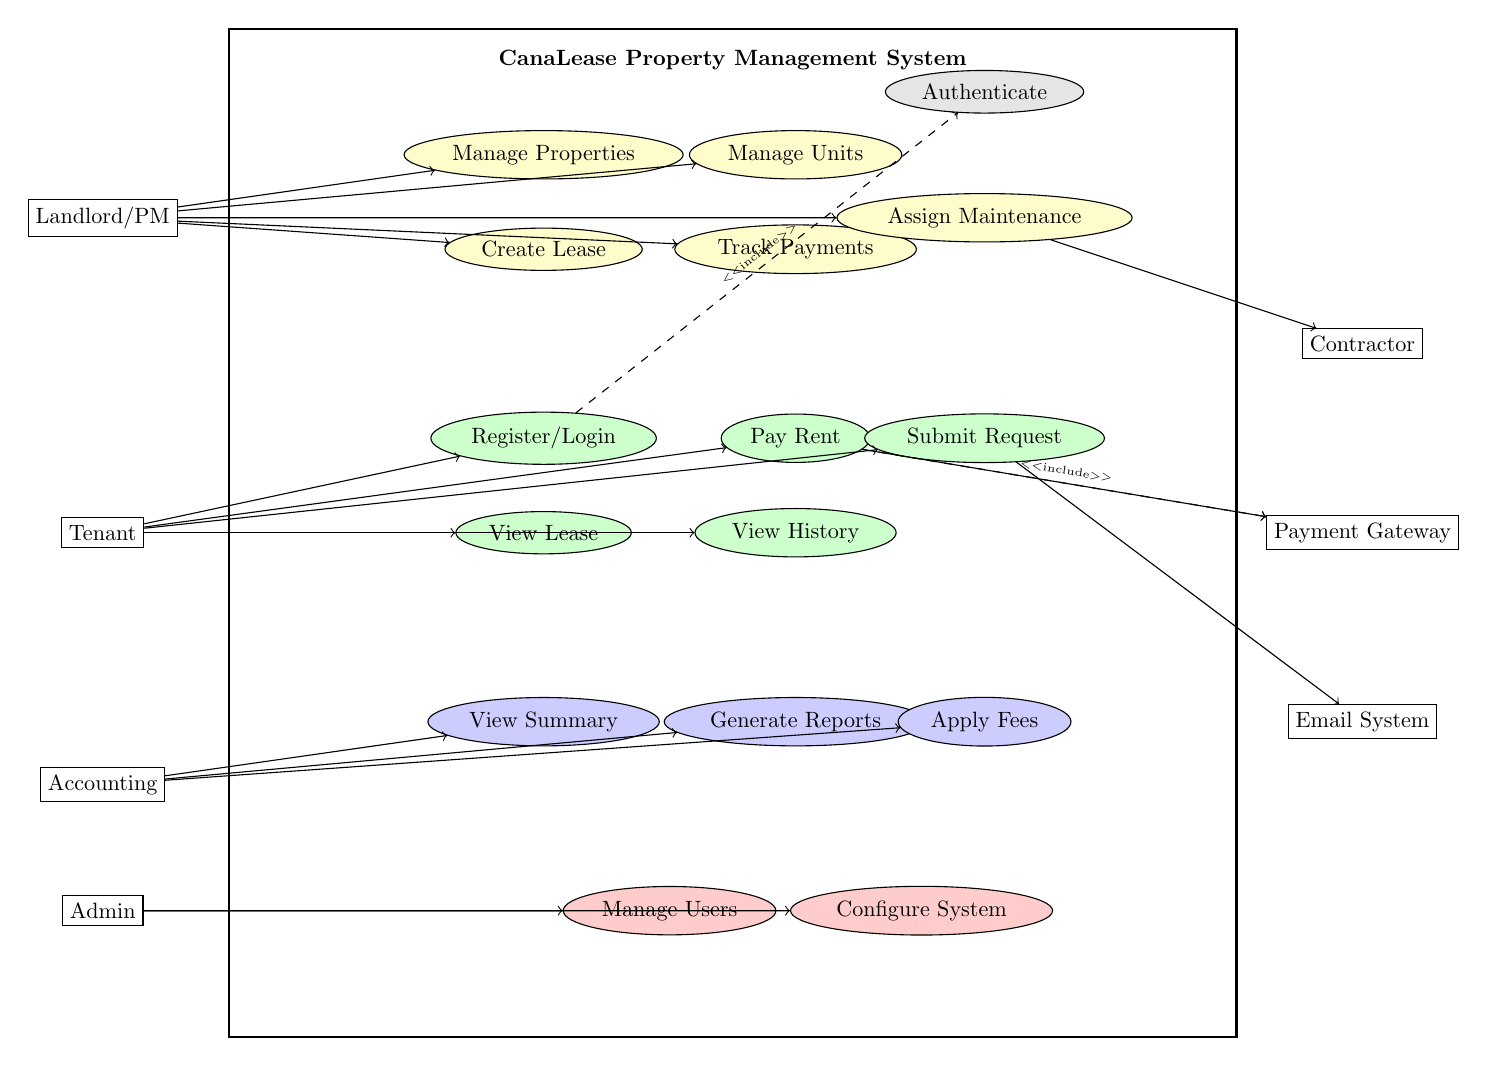
\begin{tikzpicture}[scale=0.8, transform shape]
    % System boundary
    \draw[thick] (-2,-8) rectangle (14,8);
    \node at (6,7.5) {\textbf{CanaLease Property Management System}};
    
    % Actors
    \node[draw, fill=white] (landlord) at (-4,5) {Landlord/PM};
    \node[draw, fill=white] (tenant) at (-4,0) {Tenant};
    \node[draw, fill=white] (accounting) at (-4,-4) {Accounting};
    \node[draw, fill=white] (admin) at (-4,-6) {Admin};
    \node[draw, fill=white] (contractor) at (16,3) {Contractor};
    \node[draw, fill=white] (payment) at (16,0) {Payment Gateway};
    \node[draw, fill=white] (email) at (16,-3) {Email System};
    
    % Use Cases - Landlord
    \node[ellipse, draw, fill=yellow!20] (uc1) at (3,6) {Manage Properties};
    \node[ellipse, draw, fill=yellow!20] (uc2) at (7,6) {Manage Units};
    \node[ellipse, draw, fill=yellow!20] (uc3) at (3,4.5) {Create Lease};
    \node[ellipse, draw, fill=yellow!20] (uc4) at (7,4.5) {Track Payments};
    \node[ellipse, draw, fill=yellow!20] (uc5) at (10,5) {Assign Maintenance};
    
    % Use Cases - Tenant
    \node[ellipse, draw, fill=green!20] (uc10) at (3,1.5) {Register/Login};
    \node[ellipse, draw, fill=green!20] (uc11) at (7,1.5) {Pay Rent};
    \node[ellipse, draw, fill=green!20] (uc12) at (10,1.5) {Submit Request};
    \node[ellipse, draw, fill=green!20] (uc13) at (3,0) {View Lease};
    \node[ellipse, draw, fill=green!20] (uc14) at (7,0) {View History};
    
    % Use Cases - Accounting
    \node[ellipse, draw, fill=blue!20] (uc18) at (3,-3) {View Summary};
    \node[ellipse, draw, fill=blue!20] (uc19) at (7,-3) {Generate Reports};
    \node[ellipse, draw, fill=blue!20] (uc20) at (10,-3) {Apply Fees};
    
    % Use Cases - Admin
    \node[ellipse, draw, fill=red!20] (uc24) at (5,-6) {Manage Users};
    \node[ellipse, draw, fill=red!20] (uc25) at (9,-6) {Configure System};
    
    % Include/Extend relationships
    \node[ellipse, draw, fill=gray!20] (auth) at (10,7) {Authenticate};
    \draw[dashed, ->] (uc10) -- node[above, sloped] {\tiny <<include>>} (auth);
    \draw[dashed, ->] (uc11) -- node[above, sloped] {\tiny <<include>>} (payment);
    
    % Actor associations
    \draw[->] (landlord) -- (uc1);
    \draw[->] (landlord) -- (uc2);
    \draw[->] (landlord) -- (uc3);
    \draw[->] (landlord) -- (uc4);
    \draw[->] (landlord) -- (uc5);
    
    \draw[->] (tenant) -- (uc10);
    \draw[->] (tenant) -- (uc11);
    \draw[->] (tenant) -- (uc12);
    \draw[->] (tenant) -- (uc13);
    \draw[->] (tenant) -- (uc14);
    
    \draw[->] (accounting) -- (uc18);
    \draw[->] (accounting) -- (uc19);
    \draw[->] (accounting) -- (uc20);
    
    \draw[->] (admin) -- (uc24);
    \draw[->] (admin) -- (uc25);
    
    \draw[->] (uc5) -- (contractor);
    \draw[->] (uc11) -- (payment);
    \draw[->] (uc12) -- (email);
\end{tikzpicture}
\caption{CanaLease System Use Case Diagram}
\end{figure}

\subsection{Sequence Diagram - Registering a New Tenant with Property}

\begin{figure}[h]
\centering
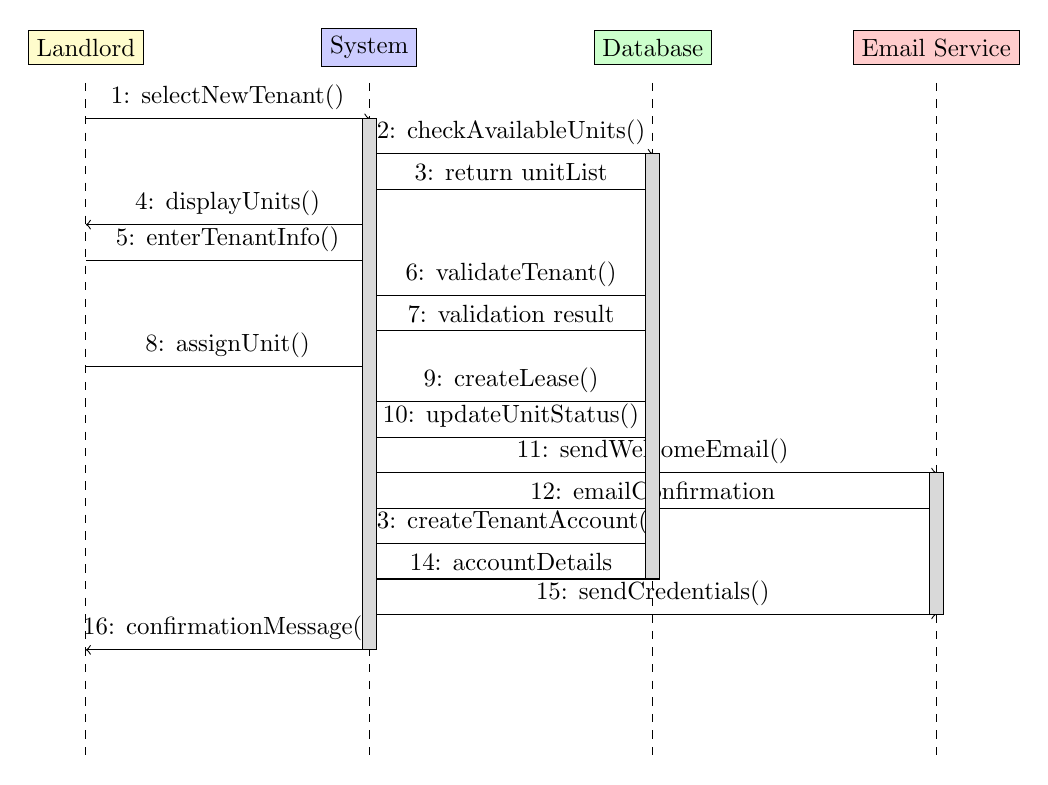
\begin{tikzpicture}[scale=0.9, transform shape]
    % Actors and objects
    \node[draw, fill=yellow!20] (landlord) at (0,0) {Landlord};
    \node[draw, fill=blue!20] (system) at (4,0) {System};
    \node[draw, fill=green!20] (database) at (8,0) {Database};
    \node[draw, fill=red!20] (email) at (12,0) {Email Service};
    
    % Lifelines
    \draw[dashed] (0,-0.5) -- (0,-10);
    \draw[dashed] (4,-0.5) -- (4,-10);
    \draw[dashed] (8,-0.5) -- (8,-10);
    \draw[dashed] (12,-0.5) -- (12,-10);
    
    % Messages
    \draw[->] (0,-1) -- (4,-1) node[midway, above] {1: selectNewTenant()};
    \draw[->] (4,-1.5) -- (8,-1.5) node[midway, above] {2: checkAvailableUnits()};
    \draw[<-] (4,-2) -- (8,-2) node[midway, above] {3: return unitList};
    \draw[<-] (0,-2.5) -- (4,-2.5) node[midway, above] {4: displayUnits()};
    
    \draw[->] (0,-3) -- (4,-3) node[midway, above] {5: enterTenantInfo()};
    \draw[->] (4,-3.5) -- (8,-3.5) node[midway, above] {6: validateTenant()};
    \draw[<-] (4,-4) -- (8,-4) node[midway, above] {7: validation result};
    
    \draw[->] (0,-4.5) -- (4,-4.5) node[midway, above] {8: assignUnit()};
    \draw[->] (4,-5) -- (8,-5) node[midway, above] {9: createLease()};
    \draw[->] (4,-5.5) -- (8,-5.5) node[midway, above] {10: updateUnitStatus()};
    
    \draw[->] (4,-6) -- (12,-6) node[midway, above] {11: sendWelcomeEmail()};
    \draw[<-] (4,-6.5) -- (12,-6.5) node[midway, above] {12: emailConfirmation};
    
    \draw[->] (4,-7) -- (8,-7) node[midway, above] {13: createTenantAccount()};
    \draw[<-] (4,-7.5) -- (8,-7.5) node[midway, above] {14: accountDetails};
    
    \draw[->] (4,-8) -- (12,-8) node[midway, above] {15: sendCredentials()};
    \draw[<-] (0,-8.5) -- (4,-8.5) node[midway, above] {16: confirmationMessage()};
    
    % Activation boxes
    \draw[fill=gray!30] (3.9,-1) rectangle (4.1,-8.5);
    \draw[fill=gray!30] (7.9,-1.5) rectangle (8.1,-7.5);
    \draw[fill=gray!30] (11.9,-6) rectangle (12.1,-8);
\end{tikzpicture}
\caption{Sequence Diagram - Registering New Tenant with Property}
\end{figure}

\subsection{Activity Diagram - Tenant Submitting Maintenance Request}

\begin{figure}[h]
\centering
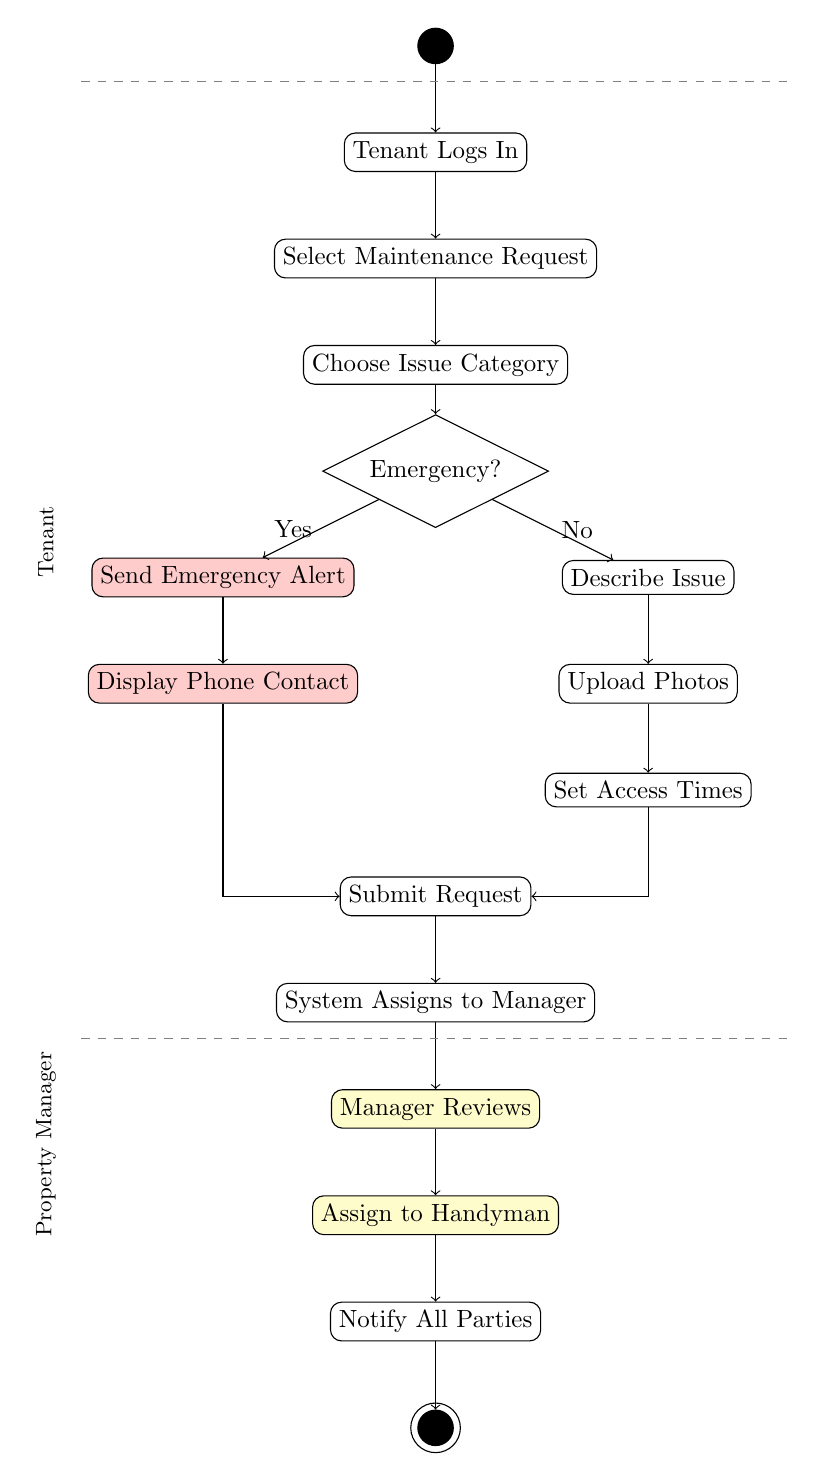
\begin{tikzpicture}[scale=0.9, transform shape]
    % Start
    \node[circle, draw, fill=black, minimum size=0.5cm] (start) at (0,0) {};
    
    % Activities
    \node[rectangle, draw, rounded corners] (login) at (0,-1.5) {Tenant Logs In};
    \node[rectangle, draw, rounded corners] (select) at (0,-3) {Select Maintenance Request};
    \node[rectangle, draw, rounded corners] (category) at (0,-4.5) {Choose Issue Category};
    
    % Decision
    \node[diamond, draw, aspect=2] (emergency) at (0,-6) {Emergency?};
    
    % Emergency path
    \node[rectangle, draw, rounded corners, fill=red!20] (alert) at (-3,-7.5) {Send Emergency Alert};
    \node[rectangle, draw, rounded corners, fill=red!20] (phone) at (-3,-9) {Display Phone Contact};
    
    % Normal path
    \node[rectangle, draw, rounded corners] (describe) at (3,-7.5) {Describe Issue};
    \node[rectangle, draw, rounded corners] (upload) at (3,-9) {Upload Photos};
    \node[rectangle, draw, rounded corners] (schedule) at (3,-10.5) {Set Access Times};
    
    % Merge
    \node[rectangle, draw, rounded corners] (submit) at (0,-12) {Submit Request};
    \node[rectangle, draw, rounded corners] (assign) at (0,-13.5) {System Assigns to Manager};
    \node[rectangle, draw, rounded corners, fill=yellow!20] (review) at (0,-15) {Manager Reviews};
    \node[rectangle, draw, rounded corners, fill=yellow!20] (assignwork) at (0,-16.5) {Assign to Handyman};
    \node[rectangle, draw, rounded corners] (notify) at (0,-18) {Notify All Parties};
    
    % End
    \node[circle, draw, fill=black, inner sep=0pt, minimum size=0.5cm] (end) at (0,-19.5) {};
    \node[circle, draw, minimum size=0.7cm] at (0,-19.5) {};
    
    % Flows
    \draw[->] (start) -- (login);
    \draw[->] (login) -- (select);
    \draw[->] (select) -- (category);
    \draw[->] (category) -- (emergency);
    \draw[->] (emergency) -- node[left] {Yes} (alert);
    \draw[->] (alert) -- (phone);
    \draw[->] (emergency) -- node[right] {No} (describe);
    \draw[->] (describe) -- (upload);
    \draw[->] (upload) -- (schedule);
    \draw[->] (phone) |- (submit);
    \draw[->] (schedule) |- (submit);
    \draw[->] (submit) -- (assign);
    \draw[->] (assign) -- (review);
    \draw[->] (review) -- (assignwork);
    \draw[->] (assignwork) -- (notify);
    \draw[->] (notify) -- (end);
    
    % Swimlanes
    \draw[dashed, gray] (-5,-0.5) -- (5,-0.5);
    \draw[dashed, gray] (-5,-14) -- (5,-14);
    \node[rotate=90] at (-5.5,-7) {\small Tenant};
    \node[rotate=90] at (-5.5,-15.5) {\small Property Manager};
\end{tikzpicture}
\caption{Activity Diagram - Maintenance Request Process}
\end{figure}

\subsection{State Machine Diagram - Applying Late Fees and Penalties}

\begin{figure}[h]
\centering
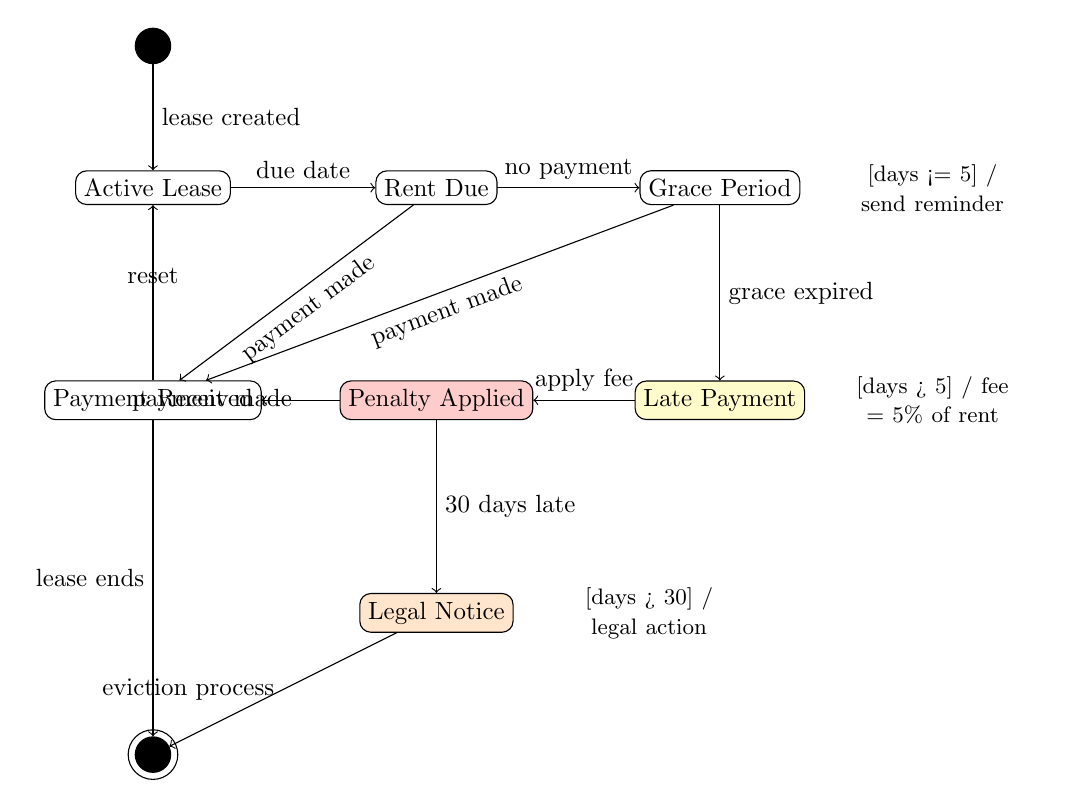
\begin{tikzpicture}[scale=0.9, transform shape]
    % States
    \node[circle, draw, fill=black, minimum size=0.5cm] (start) at (0,0) {};
    
    \node[rectangle, draw, rounded corners] (active) at (0,-2) {Active Lease};
    \node[rectangle, draw, rounded corners] (due) at (4,-2) {Rent Due};
    \node[rectangle, draw, rounded corners] (grace) at (8,-2) {Grace Period};
    \node[rectangle, draw, rounded corners, fill=yellow!20] (late) at (8,-5) {Late Payment};
    \node[rectangle, draw, rounded corners, fill=red!20] (penalty) at (4,-5) {Penalty Applied};
    \node[rectangle, draw, rounded corners] (paid) at (0,-5) {Payment Received};
    \node[rectangle, draw, rounded corners, fill=orange!20] (notice) at (4,-8) {Legal Notice};
    
    \node[circle, draw, fill=black, inner sep=0pt, minimum size=0.5cm] (end) at (0,-10) {};
    \node[circle, draw, minimum size=0.7cm] at (0,-10) {};
    
    % Transitions
    \draw[->] (start) -- node[right] {lease created} (active);
    \draw[->] (active) -- node[above] {due date} (due);
    \draw[->] (due) -- node[above] {no payment} (grace);
    \draw[->] (grace) -- node[right] {grace expired} (late);
    \draw[->] (late) -- node[above] {apply fee} (penalty);
    \draw[->] (penalty) -- node[left] {payment made} (paid);
    \draw[->] (paid) -- node[above] {reset} (active);
    \draw[->] (due) -- node[below, sloped] {payment made} (paid);
    \draw[->] (grace) -- node[below, sloped] {payment made} (paid);
    \draw[->] (penalty) -- node[right] {30 days late} (notice);
    \draw[->] (notice) -- node[left] {eviction process} (end);
    \draw[->] (paid) -- node[left] {lease ends} (end);
    
    % Guards and actions
    \node[text width=3cm, align=center] at (11,-2) {\small [days <= 5] / send reminder};
    \node[text width=3cm, align=center] at (11,-5) {\small [days > 5] / fee = 5\% of rent};
    \node[text width=3cm, align=center] at (7,-8) {\small [days > 30] / legal action};
\end{tikzpicture}
\caption{State Machine Diagram - Late Fee Application Process}
\end{figure}


% SECTION 4: SUPPLEMENTARY SPECIFICATION

\section{Supplementary Specification}

\subsection{Introduction}

\subsubsection{Purpose}
This Supplementary Specification captures the CanaLease system requirements that are not readily captured in the use cases of the use-case model. It includes legal and regulatory requirements, quality attributes, and other requirements such as operating environments and design constraints.

\subsubsection{Scope}
This document applies to the CanaLease Property Management Platform, covering all non-functional requirements that affect system design, implementation, and operation in the Canadian rental market context.

\subsubsection{Definitions, Acronyms and Abbreviations}
\begin{itemize}
    \item \textbf{MTBF:} Mean Time Between Failures
    \item \textbf{MTTR:} Mean Time To Repair
    \item \textbf{PCI DSS:} Payment Card Industry Data Security Standard
    \item \textbf{WCAG:} Web Content Accessibility Guidelines
    \item \textbf{RTO:} Recovery Time Objective
    \item \textbf{RPO:} Recovery Point Objective
    \item \textbf{CRA:} Canada Revenue Agency
\end{itemize}

\subsubsection{References}
\begin{itemize}
    \item Vision Document - CanaLease v2.0
    \item Use Case Model - Section 2 of this document
    \item Canadian Provincial Tenancy Acts
    \item PIPEDA Compliance Guidelines
\end{itemize}

\subsection{Functionality}
Additional functional requirements not expressed in use cases:

\subsubsection{Report Templates}
\begin{itemize}
    \item System shall provide T776 Statement of Real Estate Rentals format for tax reporting
    \item Monthly rent roll reports with customizable columns
    \item Vacancy reports showing unit turnover rates
    \item Maintenance cost analysis by property and category
\end{itemize}

\subsubsection{Receipt Formats}
\begin{itemize}
    \item Official rent receipts must include: landlord name, tenant name, property address, payment date, amount, period covered
    \item Receipts must be available in both English and French
    \item System shall generate CRA-compliant year-end rental receipts
\end{itemize}

\subsubsection{Calculation Formulas}
\begin{itemize}
    \item Late fee calculation: Base rent × 0.05 (5\%) after grace period
    \item Proration formula: (Monthly rent ÷ Days in month) × Days occupied
    \item Security deposit interest: As per provincial regulations (e.g., Ontario: Bank of Canada rate)
\end{itemize}

\subsection{Usability}

\subsubsection{Training Requirements}
\begin{itemize}
    \item \textbf{Indicator 1:} New landlords shall become proficient with basic operations within 2 hours of training
    \item \textbf{Indicator 2:} Tenants shall successfully complete rent payment on first attempt 95\% of the time without support
\end{itemize}

\subsubsection{Measurable Task Times}
\begin{itemize}
    \item Creating a new lease agreement: < 10 minutes for experienced users
    \item Processing rent payment: < 2 minutes
    \item Submitting maintenance request: < 3 minutes
    \item Generating monthly financial report: < 30 seconds
\end{itemize}

\subsubsection{Interface Standards}
\begin{itemize}
    \item Conform to WCAG 2.1 Level AA accessibility standards
    \item Support responsive design for screens 320px to 4K resolution
    \item Maintain consistent navigation across all modules
    \item Provide contextual help on all forms
\end{itemize}

\subsection{Reliability}

\subsubsection{Availability}
\begin{itemize}
    \item \textbf{Indicator 1:} System availability of 99.9\% (8.76 hours maximum downtime per year)
    \item \textbf{Indicator 2:} Scheduled maintenance windows limited to 4 hours per month during 2-6 AM EST
\end{itemize}

\subsubsection{Mean Time Between Failures (MTBF)}
\begin{itemize}
    \item Target MTBF: 720 hours (30 days) for critical components
    \item Payment processing module: 2,160 hours (90 days)
\end{itemize}

\subsubsection{Mean Time To Repair (MTTR)}
\begin{itemize}
    \item Critical failures (payment processing, authentication): < 2 hours
    \item Major failures (reporting, messaging): < 4 hours
    \item Minor failures (UI issues, non-critical features): < 24 hours
\end{itemize}

\subsubsection{Accuracy}
\begin{itemize}
    \item Financial calculations accurate to 2 decimal places
    \item Zero tolerance for payment processing errors
    \item Date/time accuracy synchronized with NTP servers
\end{itemize}

\subsubsection{Bug Rates}
\begin{itemize}
    \item Critical bugs: 0 per release
    \item Major bugs: < 2 per 10,000 lines of code
    \item Minor bugs: < 5 per 10,000 lines of code
\end{itemize}

\subsection{Performance}

\subsubsection{Response Times}
\begin{itemize}
    \item \textbf{Indicator 1:} Page load time: < 2 seconds for 95\% of requests
    \item \textbf{Indicator 2:} Database queries: < 100ms for simple queries, < 1 second for complex reports
\end{itemize}

\subsubsection{Throughput}
\begin{itemize}
    \item Support 1,000 concurrent transactions per second
    \item Process 50 payment transactions per second
    \item Generate 100 reports per minute
\end{itemize}

\subsubsection{Capacity}
\begin{itemize}
    \item Support 10,000 concurrent users
    \item Store 1 million property records
    \item Maintain 7 years of historical data online
    \item Handle 100,000 maintenance requests per month
\end{itemize}

\subsubsection{Resource Utilization}
\begin{itemize}
    \item CPU usage: < 70\% under normal load
    \item Memory: < 4GB per application instance
    \item Database storage: 100GB initial, scalable to 1TB
    \item Network bandwidth: 100 Mbps minimum
\end{itemize}

\subsection{Supportability}

\subsubsection{Coding Standards}
\begin{itemize}
    \item \textbf{Indicator 1:} Follow PSR-12 coding standard for PHP components
    \item \textbf{Indicator 2:} Maintain minimum 80\% code coverage in unit tests
\end{itemize}

\subsubsection{Naming Conventions}
\begin{itemize}
    \item Database tables: snake\_case (e.g., rental\_units)
    \item API endpoints: kebab-case (e.g., /api/rental-units)
    \item Classes: PascalCase (e.g., RentalUnit)
    \item Variables and functions: camelCase (e.g., getRentalUnit)
\end{itemize}

\subsubsection{Maintenance Access}
\begin{itemize}
    \item Remote diagnostic capabilities via secure VPN
    \item Administrative dashboard for system monitoring
    \item Automated error logging and reporting
    \item Database maintenance utilities for optimization
\end{itemize}

\subsubsection{Class Libraries}
\begin{itemize}
    \item Laravel framework for PHP backend
    \item React.js for frontend components
    \item Bootstrap for UI consistency
    \item Chart.js for data visualization
\end{itemize}

\subsection{Design Constraints}

\subsubsection{Technology Stack}
\begin{itemize}
    \item Backend: PHP 8.1+ with Laravel Framework
    \item Frontend: React.js 18+ with TypeScript
    \item Database: PostgreSQL 14+
    \item Cache: Redis 6+
    \item Queue: RabbitMQ for async processing
\end{itemize}

\subsubsection{Architectural Constraints}
\begin{itemize}
    \item Microservices architecture for scalability
    \item RESTful API design principles
    \item Event-driven architecture for real-time updates
    \item Multi-tenant database architecture with row-level security
\end{itemize}

\subsubsection{Purchased Components}
\begin{itemize}
    \item Moneris payment gateway integration
    \item Twilio for SMS notifications
    \item SendGrid for email delivery
    \item AWS S3 for document storage
\end{itemize}

\subsubsection{Development Tools}
\begin{itemize}
    \item Git for version control
    \item Docker for containerization
    \item Jenkins for CI/CD pipeline
    \item Jira for project management
\end{itemize}

\subsection{Online User Documentation and Help System Requirements}

\subsubsection{Documentation Requirements}
\begin{itemize}
    \item Comprehensive user manual in PDF format
    \item Interactive tutorials for new users
    \item Video guides for complex operations
    \item API documentation for integrations
\end{itemize}

\subsubsection{Help System Features}
\begin{itemize}
    \item Context-sensitive help on all screens
    \item Searchable knowledge base
    \item FAQ section organized by user role
    \item Live chat support during business hours
\end{itemize}

\subsubsection{Accessibility}
\begin{itemize}
    \item Documentation available in English and French
    \item Screen reader compatible help content
    \item Printable quick reference guides
    \item Mobile-optimized help interface
\end{itemize}

\subsection{Glossary}

\begin{itemize}
    \item \textbf{Lease:} Legal contract between landlord and tenant defining rental terms
    \item \textbf{Unit:} Individual rental space within a property
    \item \textbf{Grace Period:} Additional days after due date before late fees apply
    \item \textbf{Proration:} Calculation of partial month's rent
    \item \textbf{Security Deposit:} Advance payment held for potential damages
    \item \textbf{Work Order:} Formal request for maintenance service
    \item \textbf{Rent Roll:} Report showing all units with rental amounts and tenant information
    \item \textbf{Vacancy Rate:} Percentage of unoccupied units
    \item \textbf{PSP:} Payment Service Provider
    \item \textbf{RBAC:} Role-Based Access Control
    \item \textbf{Multi-tenancy:} Architecture supporting multiple independent customers
    \item \textbf{Escrow:} Funds held in trust by third party
\end{itemize}

% APPENDICES

\appendix

\section{Time Log}

\begin{longtable}{|p{2.5cm}|p{3cm}|p{1.5cm}|p{4cm}|p{3cm}|}
\hline
\textbf{Date} & \textbf{Task} & \textbf{Duration} & \textbf{Activity} & \textbf{Notes} \\
\hline
\endfirsthead
\hline
\textbf{Date} & \textbf{Task} & \textbf{Duration} & \textbf{Activity} & \textbf{Notes} \\
\hline
\endhead

2025-08-01 & Rebuttal Letter & 1.5h & Addressed reviewer comments & Created responses to all feedback \\
\hline
2025-08-01 & Vision Update & 2.0h & Fixed defects and inconsistencies & Updated based on D2 findings \\
\hline
2025-08-02 & Actor-Goal List & 1.0h & Identified all actors and goals & Section 2.1 \\
\hline
2025-08-02 & UC01-UC05 & 2.5h & Landlord use cases & Detailed specifications \\
\hline
2025-08-02 & UC06-UC09 & 2.0h & Landlord use cases continued & Completed landlord section \\
\hline
2025-08-03 & UC10-UC13 & 2.5h & Tenant use cases part 1 & Registration through maintenance \\
\hline
2025-08-03 & UC14-UC17 & 2.0h & Tenant use cases part 2 & Status tracking and communication \\
\hline
2025-08-03 & UC18-UC20 & 1.5h & Accounting use cases part 1 & Financial reporting \\
\hline
2025-08-04 & UC21-UC23 & 1.5h & Accounting use cases part 2 & Export and monitoring \\
\hline
2025-08-04 & UC24-UC26 & 1.5h & System admin use cases & User and system management \\
\hline
2025-08-04 & UML Diagrams & 3.0h & Created 4 required diagrams & Use case, sequence, activity, state \\
\hline
2025-08-05 & Supplementary Spec & 2.5h & Non-functional requirements & All sections completed \\
\hline
2025-08-05 & Review and Polish & 1.5h & Final review and formatting & Consistency check \\
\hline
\multicolumn{3}{|r|}{\textbf{Total Hours:}} & \textbf{25.0} & \\
\hline
\end{longtable}

\section{Traceability Matrix}

\begin{longtable}{|p{3cm}|p{4cm}|p{4cm}|p{3cm}|}
\hline
\textbf{Vision Feature} & \textbf{Use Cases} & \textbf{Supplementary Req} & \textbf{Priority} \\
\hline
\endfirsthead
\hline
\textbf{Vision Feature} & \textbf{Use Cases} & \textbf{Supplementary Req} & \textbf{Priority} \\
\hline
\endhead

Online Rent Payments & UC12, UC06, UC18 & Performance 4.5.1, Security & High \\
\hline
Lease Management & UC04, UC11 & Functionality 4.2.1, Reliability & High \\
\hline
Maintenance System & UC08, UC09, UC13, UC14 & Usability 4.3.2, Performance & High \\
\hline
Financial Reports & UC19, UC20, UC21 & Functionality 4.2.1, Accuracy & High \\
\hline
Role-Based Access & UC24, UC25 & Security, Supportability & High \\
\hline
Bilingual Support & All use cases & Usability 4.3.3, Documentation & Medium \\
\hline
Notifications & UC07, UC15 & Performance, Reliability & Medium \\
\hline
Provincial Compliance & UC04, UC22 & Functionality 4.2, Design 4.7 & High \\
\hline
Data Residency & UC26 & Design Constraints 4.7 & High \\
\hline
Seasonal Maintenance & UC08, UC09 & Functionality 4.2 & Low \\
\hline
\end{longtable}

\section{Document Revision History}

\begin{longtable}{|p{2cm}|p{2cm}|p{8cm}|p{2cm}|}
\hline
\textbf{Version} & \textbf{Date} & \textbf{Description} & \textbf{Author} \\
\hline
1.0 & 2025-07-11 & Initial Vision Document (D1) & C. Singh \\
\hline
2.0 & 2025-07-25 & Requirements Evaluation \& Risk Analysis (D2) & C. Singh \\
\hline
3.0 & 2025-08-05 & Complete SRS with Use Cases and Supplementary Specification (D3) & C. Singh \\
\hline
\end{longtable}

\end{document}